\documentclass[a4paper]{report}
\usepackage[utf8]{inputenc}
\usepackage[italian]{babel}
\usepackage{amsmath}
\usepackage{amsfonts}
\usepackage{tikz}
\usepackage{amssymb}
\usepackage{color}
\usepackage[left=1.5cm,right=1.5cm,top=1.5cm,bottom=1.5cm]{geometry}
\usepackage{listings}
\author{}
\date{}


% WATERFALL XP: solo quando tutti hanno completato deve funzionare
% MoSCoW: divido in sottogruppi e facciamo le cose insieme. ogni sottogruppo fa app separate e ad ogni step le unisco

\begin{document}

    \chapter*{Caratteristiche Generali}

        \paragraph{Specifiche progettuali}
            \subparagraph{Code Rules:} 
            \begin{itemize}
                \item utilizzare upperCamelCase
                \item nominare variabili logicamente esplicative
                \item dichiarare metodi e funzioni, variabili e costanti in italiano
                \item commentare con commento inline sopra ogni funzione/metodo specificando cosa prende in input e cosa restituisce
                \item nominare funzioni/metodi di test (ovvero funzioni che restituiscono un bool) come \emph{test[nomefunzione]} (es. testPieno)
                \item commentare con commento inline sopra ogni classe cosa rappresenta e le funzionalità che offre
            \end{itemize}
        
            \subparagraph{Metodologia:} RAD in cui per ogni 45 minuti di programmazione, i membri del gruppo si consultano per 15 minuti

        \paragraph{Il Portale e il Plebeo}
        Ti trovi nel Medioevo e hai bisogno di un Miracolo? Il Pregaverso è con te.
        
        Il Pregaverso è un portale a cui si può accedere necessariamente pagando una somma in baiocchi alla struttura di riferimento, 
        e che ci permette di acquistare servizi o beni che probabilmente verranno riscattati all'esterno del Pregaverso.

        Ovviamente l'accesso è altamente tassato e sono ben accetti solo benestanti, con ampio Credo e tasche.

        \paragraph{Feature}
            \subparagraph{Accesso Sacerdote:} il Sacerdote ha la possibilità di entrare nel Pregaverso e dare dei baiocchi iniziali al Plebeo che accederà subito dopo.
            \subparagraph{Accesso Plebeo:} il Plebeo ha la possibilità di entrare nel Pregaverso per spendere i suoi baiocchi o per pregare in modo da riceverne altri. I Plebei poveri non si meritano la permanenza.
            \subparagraph{Compra Miracolo:} il Plebeo ha la possibilità di comprare un Miracolo spendendo baiocchi, anche se l'esito è incerto e dipendente dalle tasche del Plebeo.
            \subparagraph{Prega:} il Plebeo può pregare per un certo tempo e guadagnare così baiocchi (virtuali ovviamente). Il Plebeo verrà messo in attesa e al termine della preghiera verranno depositati i baiocchi.
        
        \newpage

        \paragraph{AppMap}
            L'accesso al Pregaverso è ottenibile tramite un pagamento in baiocchi al sacerdote nella vita terrena.

            Una schermata iniziale ti darà il benvenuto nel Pregaverso. Di seguito il sacerdote della struttura a cui ti sei riferito, e a cui hai consegnato i tuoi baiocchi effettuerà l'Accesso Sacerdote.

            L'Accesso Sacerdote permette la comunicazione col Divino e soprattutto l'assegnazione nel Pregaverso dei baiocchi appena consegnati.

            Dopo aver stabilito la connessione col Divino, il Plebeo può accedere con le sue credenziali ed entrare nel Pregaverso.

            All'interno del Pregaverso è possibile comprare un Miracolo spendendo, oppure pregare per guadagnare. Al termine dei baiocchi si uscirà dal Pregaverso.

            \vspace*{1cm}

            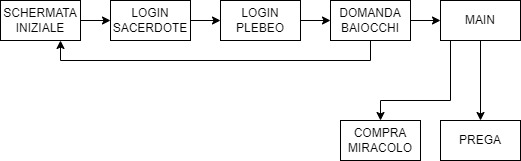
\includegraphics[scale=0.95]{sitemap.jpg}

    \chapter*{Implementazione}

            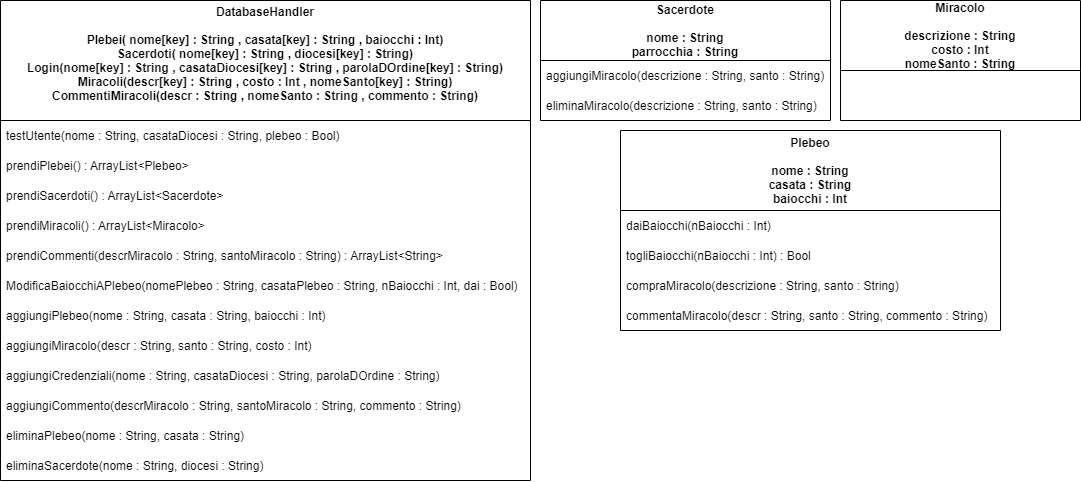
\includegraphics[scale = 0.5]{diagrammaER.jpg}

            \paragraph*{Classe Sacerdote}

                \subparagraph*{aggiungiMiracolo$($descrizione : String, santo : String$)$}
                
                \begin{verbatim}
                fun eliminaMiracolo(descrizione : String, santo : String)
                \end{verbatim}

            \paragraph*{Classe Plebeo}

                

            \paragraph*{Classe Database}

                \begin{verbatim}
                fun prendiPlebei(): ArrayList<Plebeo>
                \end{verbatim}
                Restituisce la lista di tutti i Plebei presenti al momento della chiamata all'interno del Database.
                Se non ci sono Plebei, restituisce una lista di Plebei vuota.

                \vspace*{1cm}

                \begin{verbatim}
                fun prendiSacerdoti() : ArrayList<Sacerdote>
                \end{verbatim}
                Restituisce la lista di tutti i Sacerdoti presenti al momento della chiamata all'interno del Database.
                Se non ci sono Sacerdoti, restituisce una lista di Sacerdoti vuota.

                \vspace*{1cm}

                \begin{verbatim}
                fun prendiMiracoli() : ArrayList<Miracolo>
                \end{verbatim}
                Restituisce la lista di tutti i Miracoli presenti al momento della chiamata all'interno del Database.
                Se non ci sono Miracoli, restituisce una lista di Miracoli vuota.

                \vspace*{1cm}

                \begin{verbatim}
                fun aggiungiBaiocchiAPlebeo(nome : String, casata : String, nBaiocchi : Int) : Boolean
                \end{verbatim}
                Aggiunge nBaiocchi al Plebeo univocamente identificato dalla coppia {nome,casata} all'interno del Database.
                Restituisce false se non ha modificato nessun Plebeo, se ha modificato troppi Plebei o se c'e' stato un errore sconosciuto.
                Restituisce true in caso di corretta modifica.

                \vspace*{1cm}

                \begin{verbatim}
                fun aggiungiPlebeo(nome : String, casata : String, nBaiocchi : Int) : Boolean
                \end{verbatim}
                Inserisce un nuovo Plebeo con nome nome, casata casata e con un numero di Baiocchi pari a nBaiocchi.
                Restituisce false non sono stati passati input validi.
                Restituisce true in caso di corretto inserimento.

                \vspace*{1cm}

                \begin{verbatim}
                fun aggiungiCredenziali(nome : String, casataDiocesi : String, parolaDOrdine : String) : Boolean
                \end{verbatim}
                Inserisce un nuovo utente (Plebeo o Sacerdote) con nome, casata/diocesi e Parola d'ordine.
                Restituisce FALSE se l'input è vuoto oppure già presente.
                Restituisce TRUE in caso di corretto inserimento.

                \vspace*{1cm}

                \begin{verbatim}
                fun aggiungiCommento(descrMiracolo: String, santoMiracolo : String, commento : String) : Boolean
                \end{verbatim}
                Inserisce un nuovo commento ad un miracolo con descrizione miracolo, santo del miracolo ed il commento testuale.
                Restituisce FALSE se l'input del commento è vuoto o in caso di errore generico sull'inserimento.
                Restituisce TRUE in caso di corretto inserimento.

                \vspace*{1cm}
                
                \begin{verbatim}
                fun eliminaPlebeo(nome : String, casata : String) : Boolean
                \end{verbatim}
                Elimina un Plebeo con nome nome e casata casata dal Database.
                Restituisce false se gli input non sono validi, se non ha eliminato niente o se ha eliminato piu' di una riga.
                Restituisce true in caso di eliminazione di un Plebeo (non assicura la correttezza della scelta dell'eliminato).

                \vspace*{1cm}
                
                \begin{verbatim}
                fun svuotaDatabase()
                \end{verbatim}
                Svuota completamente tutte le tabelle del database. Utile nelle funzioni di Test.

                \vspace*{1cm}
                
                \begin{verbatim}
                fun eliminaSacerdote(nome : String, diocesi : String): Boolean
                \end{verbatim}
                Elimina un Sacerdote con nome nome e diocesi diocesi dal Database.
                Restituisce false se gli input non sono validi, se non ha eliminato niente o se ha eliminato piu' di una riga.
                Restituisce true in caso di eliminazione di un Sacerdote (non assicura la correttezza della scelta dell'eliminato).

                \vspace*{1cm}
                
                \begin{verbatim}
                fun eliminaMiracolo(descr : String, nomeSanto : String): Boolean
                \end{verbatim}
                Da finire.
                Lorenzo Borgia.

                \vspace*{1cm}

\end{document}